\documentclass[12pt]{article}

\usepackage{sbc-template}

\usepackage{graphicx,url}

\usepackage[brazil]{babel}   
\usepackage[latin1]{inputenc}  
\usepackage{listings}
\usepackage{subfigure}
\usepackage{cite}
\usepackage{multicol}


     
\sloppy

\newcommand{\epos}{\textsc{Epos}}

\newcommand{\qos}{QoS}
\newcommand{\QoS}{quality of service}

\newcommand{\ov}{\emph{overhead}}
\newcommand{\ovs}{\emph{overheads}}
%\newcommand{\ov}{sobrecusto}
%\newcommand{\ovs}{sobrecustos}

\newcommand{\deadline}{\emph{deadline}}
\newcommand{\deadlines}{\emph{deadlines}}

\newcommand{\thr}{\emph{threshold}}
\newcommand{\Thr}{\emph{Threshold}}

\newcommand{\tos}{TinyOS}
\newcommand{\mos}{Mantis OS}
\newcommand{\sos}{SOS}
%\newcommand{\wsn}{rede de sensor sem fio}
%\newcommand{\wsns}{redes de sensores sem fio}
\newcommand{\wsn}{Wireless Sensor Networks}
\newcommand{\wsns}{Wireless Sensor Networks}

\lstloadlanguages{[ANSI]C++}
\lstdefinelanguage{XML} {
  keywords={xml,version,DOCTYPE,SYSTEM,EPOSConfig,family,member,name,type,
  feature,trait,class,performance,codesize,energy,power,default,pos,pre}}
\lstdefinestyle{prg} {basicstyle=\small\sffamily, lineskip=-0.2ex}
\lstdefinestyle{prgbox} {basicstyle=\small\sffamily lineskip=-0.2ex}
\lstdefinestyle{inlineprg} {basicstyle=\small\sffamily}

\newcommand{\prg}[4][htbp]{
  \begin{figure}[#1]
    \linespread{1}
    \vspace{\parskip}
    \makebox[\textwidth][c]{
      \lstinputlisting[language=#2,style=prg]{prg/#3.prg} }
    \vspace{0.4\parskip}
    \caption{#4\label{prg:#3}}
  \end{figure}
}



%\title{Uso das T�cnicas da Computa��o Imprecisa para a Ger�ncia de Energia em Sistemas Embarcados}

\title{Using Imprecise Computation Techniques for Power Management in Real-Time Embedded Systems}

\author{Geovani R. Wiedenhoft, Ant�nio A. Fr�hlich}
%\author{Luciana P. Nedel\inst{1}, Rafael H. Bordini\inst{2}, Fl�vio Rech
%  Wagner\inst{1}, Jomi F. H�bner\inst{3} }


\address{Laboratory for Software and Hardware Integration\\
Federal University of Santa Catarina\\
  PO Box 476 -- 88049-900 -- Florian\'{o}polis, SC, Brazil\\
    \email{\{grw,guto\}@lisha.ufsc.br}
}

\begin{document} 

\maketitle

\begin{abstract}


Embedded systems present severe limitations in terms of processing and memory
capabilities and are often powered by batteries, making energy 
an important resource to be managed. This work explores energy as
a parameter for Quality of Service (QoS) of embedded systems. The goal is to
guarantee the battery lifetime specified by the application and yet preserve 
the deadlines of essential (hard real-time) tasks. We propose equations to
check at project-time if a given set of tasks are schedulable. At execution-time, a
preemptive scheduler for imprecise tasks based on the Earliest-Deadline First (EDF) algorithm 
prevents the optional subtasks execution when ever there is the possibility of  
deadline loss or battery exhaustion.
A prototype was developed in \epos{} 
%(\emph{Embedded Parallel Operating System}) 
using power management mechanisms provided by the system.


\end{abstract}

%\begin{resumo} 

%Os sistemas embarcados apresentam rigorosas limita��es em rela��o �s 
%capacidades 
%de processamento e mem�ria e, por muitas vezes, s�o alimentados por baterias, o
%que torna o consumo de energia uma outra importante limita��o a ser gerenciada.
%Este trabalho explora a energia como par�metro da \QoS{} de sistemas embarcados.
%O objetivo � garantir o tempo de dura��o da bateria especificado pela aplica��o,
%com a execu��o e garantia dos \deadlines{} de, no m�nimo, tarefas priorit�rias
%especificadas previamente. Nesse contexto, n�s propomos equa��es que verificam
%em tempo de projeto se as tarefas s�o escalon�veis. Em tempo de execu��o um
%escalonador preemptivo para tarefas imprecisas baseado no algoritmo 
%\textsc{EDF} impede que as tarefas executem suas partes opcionais caso os 
%\deadlines{} das partes obrigat�rias ou o tempo de dura��o da bateria possam n�o
%ser atendidos. Um prot�tipo foi desenvolvido no \epos{} (\emph{Embedded Parallel
%Operating System}) com a utiliza��o de seus mecanismos de ger�ncia de energia.


%\end{resumo}


\section{Introduction}
% Reprogramao, estrutura + protocolo
% O que  um protocolo de disseminao
% Importncia de um prot. de diss.
% Importncia de uma boa estrutura
% Ex. de uso: reprogramao RSSF
% Contribuio: infra-estrutura p/ disseminao e reprogramao
% Organizao do artigo

%Reprogramming the software of a program in execution is a feature present in most computer environments.
%A wide range of applications make use of some reprogramming method: from internet browsers to dedicated systems, as controllers in vehicles for instance.
%Due to the limited resources of embedded systems, the software reprogramming infrastructure is different from that implemented in conventional computer environments.
%Moreover, some of these dedicated systems, as Wireless Sensor Networks (WSNs), are formed by a big amount of nodes, in which collecting and reprogramming all nodes is impractical. 

%Wireless Sensor Networks (WSN), are typically formed by a big amount of nodes, in which collecting and reprogramming all nodes is impractical.
A software reprogramming infrastructure for a Wireless Sensor Network (WSN) is composed of a data dissemination protocol and a structure capable of organizing the data in the system's memory. By using an embedded Operating System (OS) it is possible to provide for embedded applications an infrastructure to hide this data organization. Usually, the reprogramming structures present in OSs are composed of updatable modules. These modules are memory position independent and are replaced at runtime~\cite{sos}~\cite{contiki}. 

In addition, it is essential that all new data of one or more modules is correctly received by all nodes involved in the reprogramming process. In order to provide safe data transfer, a data dissemination protocol is used together with the OS infrastructure.
%In general, a dissemination protocol works as follows: the dissemination begins from a base station responsible to transfer the new data to its neighbor nodes. Once a node receives the new data, it is capable of retransmitting it to its own neighbors.  The process repeats until the entire network is up to date~\cite{moap}~\cite{deluge}.
%Thus, if a node A is neighbor of a node B, and the node B has A and C as neighbors, the node B after receiving the new data from the node A will retransmit it to the node C. The process repeats for all nodes until the entire network is up to date~\cite{moap, deluge}.

Epos Live Update System (\ELUS{}) is an OS infrastructure for software updating that has better performance in terms of memory consumption, method invocation time, and reconfiguration time when compared to related works~\cite{Gracioli:2010}.
%Although this favorable result, we identifed that memory consumption of \ELUS{} could be improved.
Although this favorable result, \ELUS{} memory consumption could still be improved.
Furthermore, \ELUS{} does not have any support for data dissemination. 

%In summary, in this paper, we make the following contributions:
%\begin{itemize}
%	\item We improved the memory consumption of \ELUS{} by using C++ templates specialization techniques (more than 50\% of improvement). %\ELUS{} is implemented around the EPOS metaprogrammed framework~\cite{Frohlich:2001}. Thus, some code regions are duplicated due to the use of templates. We identified some of these regions and applied a template specialization technique~\cite{stroustrup:2000}.
%	\item We provide a domain engineering analysis considering the data dissemination protocols characteristics. The protocols characteristics are decomposed into a feature diagram that shows common and variable features present in different protocols.
%	\item We integrate a data dissemination protocol to \ELUS{} and evaluate the new infrastructure in terms of memory consumption and dissemination and reprogramming times. %As result, we provide a lightweight software reprogramming infrastructure for resource-constrained embedded systems.
%\end{itemize}

%In this paper we make the following contributions: (i) we have improved the memory consumption of \ELUS{} by using C++ templates specialization techniques; (ii) we provide a data dissemination protocol domain engineering analysis considering protocols characteristics, and integrate our developed protocol to \ELUS{}; and (iii) we evaluate the new infrastructure in terms of memory consumption, and dissemination and reprogramming times.
In this paper we make the following contributions: (i) we develop and integrate a data dissemination protocol to \ELUS{}; (ii) we improve the memory consumption of \ELUS{} by using C++ templates specialization techniques; and (iii) we evaluate the new infrastructure in terms of memory consumption, and dissemination and reprogramming times.

%The rest of this paper is organized as follows.
%Section~2 presents the related work.
%Section~\ref{sec:ddp} shows the designed dissemination protocol and compares its characteristics to other proposed protocols.
Section~\ref{sec:ddp} presents the design of the developed dissemination protocol.
Section~\ref{sec:integration} presents the integration between the dissemination protocol and \ELUS{}.
The evaluation of the infrastructure is carried out in Section~\ref{sec:evaluation}.
Finally, Section~\ref{sec:conc} concludes the paper.


\section{Related Work}
\label{sec:related}

Several works have addressed the deployment of energy harvesters in wireless sensor networks.
Although many of them did not take real-time constraints into account, some can be adapted to support timing requirements.
This section describes the approaches these works used in order to schedule energy usage in energy-harvesting systems.

An important factor for efficiently managing energy in energy-harvesting systems is the choice of an efficient predictor for energy input~\cite{Paradiso:2005}.
% Kansal (Heliomote)
Kansal et al.~\cite{Kansal:2007} introduced a prediction algorithm to support their power management approach for wireless sensor networks.
Their energy prediction model uses an exponentially weighted moving-average filter.
This method assumes that solar irradiation in a given time-slot of the day is similar to the irradiation in the same time-slot of other days.
Their power management approach took into account the predicted amount of energy input to maximize the duty-cycle of the system, subject to energy availability.
% Moser
Moser et al.~\cite{Moser:2007} used a similar approach.
Their work presents a system model, simulated experimental results, and a real implementation of the proposed control law.
The shown experiments, however, focus on a single sensor node, not taking wireless communication into account.
% Recas?
Ali et al.~\cite{Ali:2010} proposed an extension to these models.
Their approach take not only the past days into account, but also the solar irradiation levels of the current day.
This allows for lower prediction errors as, by monitoring the irradiation levels of the current day, it is possible to adjust predicted energy according to the most recent information, i.e., the prediction errors in the most recent time-slots.

A few works analyzed the problem of efficiently scheduling tasks in systems presenting varying energy budgets.
% Rusu:2003
Rusu et al.~\cite{Rusu:2003} presents a multiversion scheduling approach that chooses between the different versions of the same tasks that maximize the system value and prevents battery depletion.
Assuming that batteries may be recharged, they propose a static solution that maximizes value based on worst-case scenarios.
Also, they propose a dynamic scheme that takes advantage of the slack energy generated in the system when worst-case energy consumption does not take place.
% ElGhor:2011
El Ghor et al.~\cite{ELGhor:2011} proposed a modified EDF scheduler that takes energy production, storage, and consumption into account.
They show by simulation that the approach outperforms other algorithms in terms of rate of deadline misses and required size of energy storage.
% Sharma:2010
Sharma et al.~\cite{Sharma:2010} analyze the problem from a different perspective.
They consider that the function of the device in a WSN is solely to sense and to forward data through the wireless interface.
In this context, they propose a set of policies to minimize the size of an outgoing queue subject to energy availability.
They assume that, the smaller the queue size, the larger the amount of data forwarded through the network, and, consequently, the better the system quality.
% Dehghan
% - Still unpublished

From all studied related work, only Kansal et al.~\cite{Kansal:2007} have analyzed the impact of their work in terms network-wide performance.
Other works only analyze the performance of isolated energy-harvesting sensor nodes.
% For this reason, only the approach presented by Kansal and his colleagues have been considered for comparison with the results presented in this paper.

% Adaptive scheduling techniques have long been used to handle processing
% overloads in real-time systems.
% Buttazzo~\cite{Buttazzo:2011} classifies the adaptive scheduling techniques into three categories: job skipping, period adaptation, and service adaptation.
% Altought initially conceived to handle processing overloads, such techniques may also be applied to handle energy overload, once energy consumption decreases as a consequence of reducing the amount of work executed by the system.
% In fact, a few works have already explored this characteristic~\cite{a few
% works}.

% In job skipping techniques, tasks are prevented from executing when the system is overloaded~\cite{Koren:1995,Ramanathan:1995,Ramanathan:1999}.
% Period adaptation techniques alter tasks' frequencies in order to lower system utilization, hence making the system schedulable~\cite{Buttazzo:1998,Kuo:1991,Seto:1998,Abdelzaher:1997}.
% Service adaptation techniques selectively tune system quality set-points in order to be able to comply with system constraints~\cite{Liu:1991,Cucinotta:2010,Yuan:2006,Cornea:2003}.
% Regardless of the technique, systematic ways to adapt the system are deployed in order to control the impact on system quality.

% Some adaptive scheduling approaches have already been deployed in embedded systems and wireless sensor networks to ensure the lifetime of system batteries.
% Not all of them, however, take into account real-time requirements and/or the impact on system quality.

%VADC
% Wanner et al.~\cite{Wanner:2011} proposes a technique called \emph{Variability-Aware Duty Cycling} (\textsc{Vadc}) that adapts duty cycle of wireless sensors by changing task's periods.
% Besides traditional WSN power management techniques, they also take into account hardware power variability, being the duty cycle adapted to observed variations on energy consumption.
% It has a working implementation for \textsc{TinyOS} that includes abstractions for defining adaptable task parameters (period and iterations only) and system models to derive duty cycles able to guarantee a minimum battery lifetime.
% This work relate to ours in the sense that both works adapt the WSN system to guarantee that the energy demands won't ever surpass the energy availability.
% The core difference among them is that while \textsc{Vadc} considers that the energy demand varies due to hardware power variability, we consider that the energy availability varies.
% Moreover, once in our approach energy consumption is monitored at runtime, variations on energy demand are also captured, being the system also able to adapt to such demand variations. 

%Cinder
% Rumble et al.~\cite{Rumble:2009} presented a service adaptation technique based
% on resource reservation, taking energy as a manageable resource.
% The system is called \emph{Cinder}.
% They defined policies to ensure \textit{isolation}, \textit{delegation}, and \textit{subdivision} of allocated resources, doing it through an abstraction they called \emph{capacitor}.
% The system has a ``main'' capacitor (its battery) with a known charge.
% Each task is associated to a capacitor abstraction that is ``charged'' by a higher level capacitor.
% Child tasks also have capacitors, but instead of being ``charged'' by the battery, they drain resources from its parent task.
% Periodically, the system distributes resources (energy) through the capacitor tree.
% This distribution is based on a consumption rate defined as a function of required system lifetime and available energy.
% Cinder was implemented in the \textsc{HiStar} operating system for mobile phones.

%Levels
% Lachenmann et al.~\cite{Lachenmann:2007} proposed \textsc{Levels}, a service adaptation and multi-version scheduling mechanism for wireless sensing systems.
% Their objective is to maximize system quality while respecting a pre-defined requirement of battery duration lifetime.
% They focus on critical application where there is no redundancy and no node may fail before the required operation time.
% In their approach they assume a component-based system and define ``energy levels'' at which each of system components may behave in a different way, consuming less energy and decreasing system quality as the ``levels'' go down.
% At runtime, the system is adapted by setting its energy level to the one that is able to comply with de lifetime requirement given the amount of available energy.
% Levels was implemented in \textsc{TinyOS}.

%ECOSystem
% Ellis et al.~\cite{Zeng:2005} developed the \textsc{ECOSystem}, which is an operating system with support for application adaptation with focus on multimedia systems.
% Similarly to what Cinder does, they defined an abstraction for energy in the system, the \emph{currentcy}.
% In this system, authors expect the energy resource (currentcy) to be allocated in the same way other resources are (e.g., memory, i/o device), i.e., the application should explicitly allocate energy for its execution.
% Each application is allowed to use a pre-defined amount of energy.
% This amount is updated periodically based on the amount of available energy and the required working time.
% \textsc{ECOSystem} was implemented as a modified version of \textsc{Linux}.

% Table~\ref{tab:related_comparisson} shows a comparison of the presented work.
% The next section presents an approach for integrating the desired
% characteristics of the proposed framework (section~\ref{sec:obj}) and exploring
% application-driven adaptation of RT-WSN applications.

%Comparisson
%
% parameters: classe, real-time (soft/hard), mettering/account method, renewable
% energy, system variability (battery + hardware), simulation/real
% implementation/operating system, sincroniza��o, invers�o de prioridade
%
% \tab{related_comparisson}{Comparison of related work.}

%%\input{textos/motivacao}
\section{Background}
%\section{QoS: The Role of Energy}
\label{sc:proposta}

%- Atender o tempo de dura��o do sistema. Atrav�s da utiliza��o de t�cnicas da computa��o imprecisa. Parte obrigat�ria e Parte opcional... (Explicar o que � em 2 ou 3 par�grafos). 

%Este trabalho tem como proposta o desenvolvimento de uma abordagem para garantir que o tempo de vida da bateria de sistemas embarcados possa durar o tempo desejado pela aplica��o com os \deadlines{} atendidos de, no m�nimo, tarefas essenciais especificadas previamente pelo usu�rio. Para isso, nosso escalonador deve realizar diminui��es controladas dos n�veis de \qos{} da aplica��o com objetivo de economizar energia quando � detectada que a carga da bateria n�o ser� suficiente para atender o tempo especificado pela aplica��o. Neste trabalho, o controle da diminui��o dos n�veis de \qos{} da aplica��o � inspirado nos mecanismos da computa��o imprecisa~\cite{Liu:1994}, que divide as tarefas em duas partes: uma parte obrigat�ria e outra parte opcional. O escalonador proposto � baseado no algoritmo de escalonamento \textsc{EDF} (\emph{Earliest Deadline First}) com objetivo de atender os \deadlines{} das partes obrigat�rias. 

This work aims at guaranteeing that the batteries used in an embedded system
can last at least the time required by the application and yet preserving the
deadlines of essential tasks, i.e., the deadlines of hard real-time tasks.
%meeting the deadlines of essential tasks as defined by the embedded system developer. 
%This work developed an approach to guarantee that embedded systems' batteries lifetime can last time desired by application with deadlines met of at least essential 
Our scheduler
starts to decrease \qos{} levels in order to save energy when it detects
that batteries will not last long enough to satisfy a previously defined
expected system lifetime. The decreased control of application \qos{} levels is
based on imprecise computation mechanisms~\cite{Liu:1994}, which divide tasks
into two subtasks: a mandatory one and an optional one. The proposed scheduler 
is based on the \textsc{EDF} (\emph{Earliest-Deadline First}) scheduling algorithm.
%in order to meet the mandatory subtasks deadlines.

%A se��o~\ref{sc:proposta:imprecisa} descreve a computa��o imprecisa e a inspira��o para a energia. Se��o~\ref{sc:proposta:edf} aborda o algoritmo de escalonamento \textsc{EDF}. Se��o~\ref{sc:proposta:proposta} apresenta a proposta com maiores detalhes, bem como o algoritmo do escalonador e as equa��es que devem ser respeitadas para as tarefas serem escalon�veis.

% Coment�rio Lucas: este segundo �ndice t� forcado! Acho que elimina!

%Section~\ref{sc:proposta:imprecisa} describes the imprecise computation and the
%inspiration for energy. Section~\ref{sc:proposta:edf} gives an insight on
%scheduling algorithm \textsc{EDF}. Section~\ref{sc:proposta:proposta} presents
%the scheduler algorithm with more details and the equations that must be
%respected to the tasks being scalable.


\subsection{Imprecise Computation}
\label{sc:proposta:imprecisa}

%A computa��o imprecisa � uma t�cnica de escalonamento originalmente proposta para atender os requisitos temporais das tarefas de tempo real atrav�s de diminui��es controladas dos n�veis de \qos{}. O controle dos n�veis de \qos{} realizado pela computa��o imprecisa diminui a qualidade do resultado, n�o executando as partes opcionais, com objetivo de garantir que nenhum \deadline{} de execu��o das partes obrigat�rias seja perdido. 

Imprecise computation is a scheduling technique originally proposed to
satisfy timing requirements of real-time tasks through decreasing
levels of \qos{}. The control of application \qos{} levels done by imprecise
computation worsens quality of results by not executing optional subtasks 
in order to guarantee that no mandatory subtask deadlines will be lost.

%Com a divis�o de cada tarefa em duas partes, a computa��o imprecisa une a computa��o de tempo real e as t�cnicas de ``melhor esfor�o'' para, respectivamente, a parte obrigat�ria e a parte opcional. A parte obrigat�ria das tarefas gera resultados imprecisos que refletem o m�nimo de \qos{} para garantir que esses resultados sejam �teis. Os resultados imprecisos t�m suas qualidades elevadas quando as partes opcionais s�o executadas, com a gera��o de resultados precisos. 

With the division of each task into two parts, imprecise computation unites
real-time computing and ``best effort'' techniques for, respectively, the
mandatory and optional subtasks. The mandatory subtask of imprecise tasks
generates imprecise results which reflect the minimum of \qos{} to guarantee
that these results are useful. These imprecise results have their quality
enhanced when the optional subtask executes, generating the precise
results.

%
%- Explicar sobre os estados poss�veis das partes das tarefas. Figura~\ref{fig:diagramaAutomatosFinitos} � um diagrama ...
%

%A figura~\ref{fig:diagramaAutomatosFinitos} apresenta as transi��es de estados da parte obrigat�ria e da parte opcional. O estado \textit{Esperando} indica as tarefas que esperam por um novo per�odo. O estado \textit{Pronto} indica as tarefas que est�o prontas para executarem e aguardam serem escalonadas. A tarefa no estado \textit{Executando} � aquela que est� utilizando o processador. Nessa figura � poss�vel observar que a diferen�a entre as transi��es de estados da obrigat�ria e da opcional � do estado \textit{Pronto} para o estado \textit{Esperando}. Essa diferen�a indica que a parte opcional pode ser cancelada antes mesmo de ser executada, pois ela estaria no estado \textit{Pronto} e n�o no estado \textit{Executando}. Al�m disso, a parte opcional pode ser cancelada durante a execu��o, ou seja, do estado \textit{Executando} para o estado \textit{Esperando}, mesmo que n�o tenha terminado a sua execu��o. A parte obrigat�ria s� pode ir para o estado \textit{Esperando} depois que passar pelo estado \textit{Executando} e finalizar a execu��o no seu per�odo.


%Figure~\ref{fig:diagramaAutomatosFinitos} presents the state transitions of the mandatory and optional subtasks. In the \textit{WAITING} state are the tasks waiting for a new period. In the \textit{READY} state are the tasks ready to execute and waiting to be scheduled. The task in the \textit{RUNNING} is the one using the processor. It is possible to observe in this figure that the difference between mandatory and optional state transitions is from state \textit{READY} to state \textit{WAITING}. This difference indicates that the optional subtask can be canceled before to be executed, because it would be in the \textit{READY} state and not in the \textit{RUNNING} state. Moreover, the optional subtask can be canceled during the execution, i.e., from \textit{RUNNING} state to \textit{WAITING} state without to finish its execution. The mandatory subtask can only go to \textit{WAITING} state after to pass in the \textit{RUNNING} state and to finalize its execution in the period. 


%\begin{figure}[!ht]
%\centering
%     {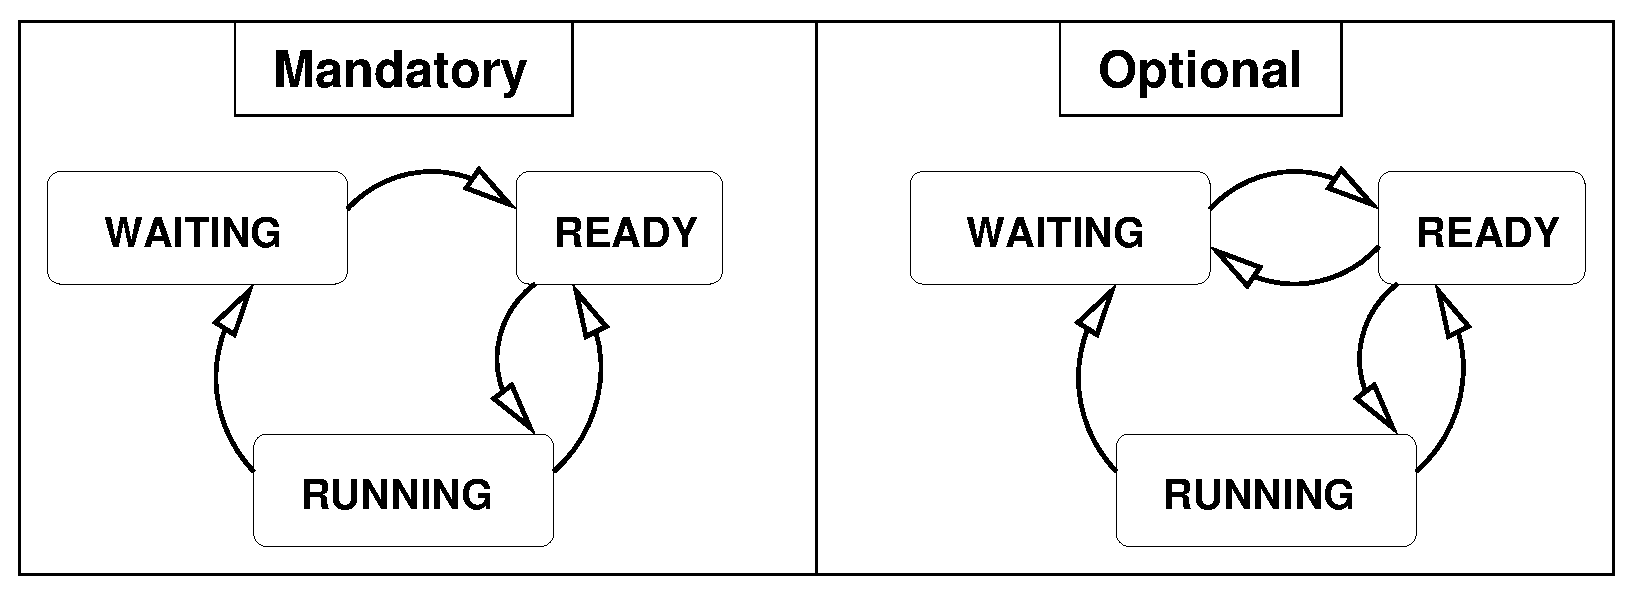
\includegraphics[scale=0.45]{figuras/statesTransitions.eps}}
%     %\caption{Transi��es de estados da parte obrigat�ria e da parte opcional.}
%     \caption{State transitions of the mandatory and optional subtasks.}
%     \label{fig:diagramaAutomatosFinitos}
%\end{figure}

%Na literatura existem diversas possibilidades de aplica��es da computa��o imprecisa, como, por exemplo, o processamento de imagens. Neste exemplo, as partes obrigat�rias gerariam uma imagem com uma qualidade m�nima aceit�vel, enquanto que as partes opcionais aumentariam a qualidade dessa imagem. Os algoritmos ``a qualquer tempo'' s�o outras possibilidades de aplica��es para a computa��o imprecisa, que incluem: os m�todos num�ricos, os c�lculos de ra�zes, os c�lculos de polin�mios, as aproxima��es num�ricas, e entre outros. Esses algoritmos, normalmente, implementam m�todos iterativos que refinam os resultados depois de cada itera��o. Nesse caso, quanto mais tempo o algoritmo � executado, melhor � a qualidade do resultado. As aplica��es de controle\&conforto s�o outras possibilidades para a computa��o imprecisa. Um exemplo � o monitoramento da temperatura de uma caldeira que pode derreter ou at� mesmo explodir caso ultrapasse uma certa temperatura. Nesse exemplo, o controle verifica em per�odos espec�ficos a temperatura da caldeira e aciona recursos para diminuir essa temperatura caso ultrapasse um valor. O conforto pode realizar c�lculos adicionais nos dados das temperaturas obtidas, como a m�dia das temperaturas analisadas em um determinado per�odo, a contagem do n�mero de vezes que a temperatura chegou a um certo n�vel, e entre outros. 
%Entretanto, em caso de sobrecarga no sistema, essas tarefas realizadas pelo ``conforto'' podem ser descartadas pelo maior grau de import�ncia das tarefas realizadas pelo ``controle''. 


Literature presents several possible applications of imprecise
computation. For instance, one can use imprecise tasks to implement image
processing systems. In this example, the mandatory subtasks should generate an
image with an acceptable quality while optional subtasks could enhance
the image quality. The ``anytime algorithms'' are other possibilities of
imprecise computation which include among others: 
numeric methods, roots calculations,
polynomials calculations and numeric approximations. These algorithms usually
implement iterative methods that refine the results after each iteration. In
this case, the longer an algorithm is executed, better is the result
quality. Another set of applications are control\&comfort applications, which
the control being the mandatory subtask and the comfort being 
the optional subtask. One example is the monitoring of the boiler temperature 
that can melt or even explode. In this example, the control verifies the
temperature and triggers resources to reduce that when the temperature exceed a
threshold. The comfort can calculate information about the sampled temperature
such as the temperatures average in a period, the number of times that
temperature exceed a threshold, and among others. 


%- Explicar a possibilidade para energia na figura~\ref{fig:energiaComputacaoImprecisa}.

%A partir desse conceito de divis�o de cada tarefa em parte obrigat�ria e parte opcional, a computa��o imprecisa mostra-se favor�vel para a utiliza��o em nossa proposta em rela��o � energia. A figura~\ref{fig:energiaComputacaoImprecisa} apresenta uma tarefa que consumiria \textsc{X} unidades de energia obrigatoriamente, e quando dividida em parte obrigat�ria (\textsc{Y} unidades de energia) e parte opcional (\textsc{Z} unidades de energia) permite a economia de \textsc{Z} unidades de energia caso a parte opcional n�o seja executada.

The imprecise computation showed us favorable to use in our proposal in relation
to energy. Suppose that a task consumes \textsc{X} energy units obligatorily.
When it is divided into mandatory subtask (\textsc{Y} energy units) and optional
subtask (\textsc{Z} energy units) the scheduler can save \textsc{Z} energy units
if the optional subtask is not executed.


%Figure~\ref{fig:energiaComputacaoImprecisa} presents a task that consumes \textsc{X} energy units obligatorily. When it is divided into mandatory subtask (\textsc{Y} energy units) and optional subtask (\textsc{Z} energy units) the scheduler can save \textsc{Z} energy units if the optional subtask is not executed. Thus, the imprecise computation show us favorable to use in our proposal in relation to energy.


%\begin{figure}[!ht]
%\centering
%     {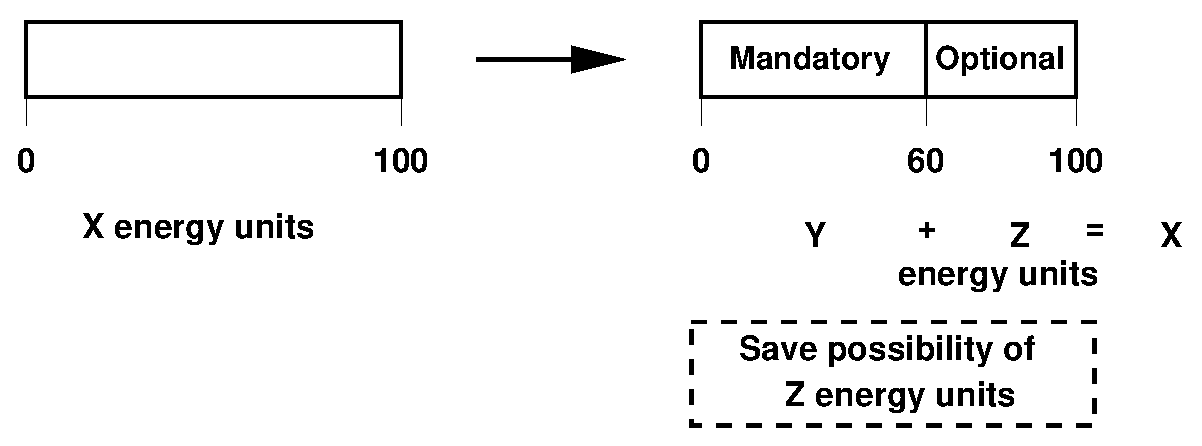
\includegraphics[scale=0.58]{figuras/energyImpreciseComputation.eps}}
%     %\caption{Computa��o imprecisa em rela��o � energia consumida.}
%     \caption{Imprecise computation in relation to energy consumed.}
%     \label{fig:energiaComputacaoImprecisa}
%\end{figure}


\subsection{\textsc{EDF}}
\label{sc:proposta:edf}


%- Utiliza��o do algoritmo EDF para atender as partes obrigat�rias. (Explicar sobre o EDF) (Posso colocar figura)

%O algoritmo \textsc{EDF} (\emph{Earliest Deadline First})~\cite{Liu:1973} � um mecanismo de escalonamento tempo real baseado em prioridades din�micas e muito utilizado na literatura. \textsc{EDF} distribui maiores prioridades para as tarefas com \deadlines{} mais curtos. Em tempo de projeto, um teste de escalonabilidade avalia a possibilidade de alguma tarefa perder o seu respectivo \deadline{}. Em tempo de execu��o, um escalonador preemptivo escolhe a tarefa em estado \textit{Pronto} de mais alta prioridade.

The \textsc{EDF} (\emph{Earliest-Deadline First})~\cite{Liu:1973} algorithm is a
real-time scheduling mechanism based on dynamic priorities and widely used in
the literature. \textsc{EDF} distributes the highest priorities to the tasks
with the shortest deadlines. At project-time a schedulability test evaluates the
possibility of any task lose its deadline. At execution-time a preemptive
scheduler selects to execute the highest priority task in \textit{READY} state.

%O modelo de tarefas para esse teste �: tarefas peri�dicas e independentes com o \deadline{} igual ao per�odo.

%Um teste de escalonabilidade exato para o algoritmo \textsc{EDF} � apresentado a seguir. O sistema de tempo real considerado cont�m $n$ tarefas peri�dicas e independentes, {\Large $\tau$} = $\{\tau_0,\tau_1,...,\tau_{n-1}\}$. Cada $\tau_i$ � caracterizado por tr�s par�metros, $(P_i, D_i, C_i)$, onde, $P_i$ � o per�odo em que a tarefa $i$ � escalonada, $D_i$ � o prazo (\emph{deadline}) m�ximo de conclus�o relativo ao instante da libera��o da tarefa $i$ e $C_i$ � o tempo de execu��o da tarefa $i$ no pior caso (inclu�do tempos de espera pela invers�o de prioridades). Para este teste � suposto que $\forall\tau_i$, $D_i=P_i$ . A utiliza��o $U_i$ de uma tarefa $i$ em termos de processamento � representada pela equa��o (\ref{eq:edf:u}).

An exact schedulability test of the \textsc{EDF} algorithm is presented below.
The real-time system considered contains $n$ periodic and independent tasks,
{\Large $\tau$} = $\{\tau_0,\tau_1,...,\tau_{n-1}\}$. Each $\tau_i$ is
characterized by three parameters, $(P_i, D_i, C_i)$, where $P_i$ is the period
in which the task $i$ is scheduled, $D_i$ is the max relative deadline of
conclusion in relation to instant of the task $i$ release and $C_i$ is the 
task $i$ execution time in the worst case which included times waiting by 
the priorities reversal.
In this test is supposed that $\forall\tau_i$, $D_i=P_i$ . The utilization $U_i$
of the task $i$ in processing terms is represented by equation (\ref{eq:edf:u}).


\begin{equation}
U_i = \frac{C_i}{D_i}
\label{eq:edf:u}
\end{equation}


%\[ U_i = \frac{C_i}{D_i} \]

%A capacidade de um processador � definida como 1, ou seja, 100\%. Um sistema com $\omega$ processadores possui capacidade $\omega$. Dessa forma, para as tarefas serem escalon�veis no algoritmo \textsc{EDF}, o somat�rio das utiliza��es de todas as tarefas deve ser menor ou igual a capacidade dos processadores, ou seja, 
The processor's capacity is set to 1, i.e., 100\%. A system with $\omega$
processors has $\omega$ capacity. Thus, in order to tasks to be schedulable 
in the \textsc{EDF} algorithm, the utilization sum of all the tasks must be less
than or equal to the processors' capacity, i.e.


\begin{equation}
\sum_{i=1}^n \left (\frac{C_i}{D_i} \right) \le \omega
\label{eq:edf:formalizacao}
\end{equation}

%\[ \sum_{i=1}^n \left (\frac{C_i}{D_i} \right) \le \omega \]

%onde $\omega = 1$ para um sistema com mono-processador. Caso $\sum_{i=1}^n U_i > \omega$, o processador estar� sobrecarregado e as tarefas n�o s�o escalon�veis nesse algoritmo.

\noindent where $\omega = 1$ on a system with mono-processor. If $\sum_{i=1}^n U_i >
\omega$ , the processor will be overloaded and the tasks will not be
schedulable.  


%\begin{figure*}[!ht]
\linespread{1}
\begin{center}
\begin{footnotesize}

\lstset{language=c++,frame=lrtb}
\lstset{basicstyle=\ttfamily}
\lstset{commentstyle=\textit}

  \begin{minipage}{14cm}
    \lstinputlisting{figuras/testeEscalonabilidadeEDF.tex}
  \end{minipage}

\caption{Teste de escalonabilidade do algoritmo \textsc{EDF}.}
\label{fig:testeEDF}
\end{footnotesize}
\end{center}
\end{figure*}




\section{Building a Trustful Infrastructure for Future Internet}
\label{sec:solution}
The Internet architecture demonstrate inefficiency and problems in several and large areas, such as mobility, real-time applications,
failures (e.g. equipment, software bugs, and configuration mistakes), and especially in pervasive security problems \cite{Rexford:2010}.
Moreover, the Internet lacks effective solutions in terms of scalability and sustainability, 
consuming much more energy and hindering the management of countless sensor devices that are so important for several applications in the Future Internet.
Hence, we propose the use of a stack of communication protocols (UDP@NDN@C-MAC), in the scope of the EPOSMote project,
designed specifically to guarantee a trustful communication
%Our solution also includes EPOSMote II, an embedded platform. Thus, 
while still compromised with the low utilization of resources (processing, memory, power and communication bandwidth).
%and the use of EPOSMote II which is an embedded platform and represents a typical Future Internet device.

\subsection{EPOSMote}
The EPOSMote is an open hardware project~\cite{eposmote}. Initially it aimed at 
the development of a wireless sensor network module, and focused on environment 
monitoring. Its first version, the EPOSMote I, features an 8-bit AVR microcontroller, 
IEEE 802.15.4 communication capability and a small set of sensors.

As the project evolved a second version arose, with the objective of delivering a 
hardware platform to allow research on energy harvesting, biointegration, and 
MEMS-based sensors. The EPOSMote II focus on modularization, and thus is composed 
by interchangeable modules for each function.

Figure \ref{emote2-block_diagram} shows an overview of the EPOSMote II architecture.
Its hardware is designed as a layer architecture composed by a main module,
a sensoring module, and a power module. The main module is responsible for processing
and communication. It is based on the Freescale MC13224V microcontroller~\cite{mc13224v}, which possess 
a 32-bit ARM7 core, an IEEE 802.15.4-compliant transceiver, 128kB of flash memory, 80kB of ROM memory
and 96kB of RAM memory. We have developed a startup sensoring module, which contains some sensors  
(temperature and accelerometer), leds, switches, and a micro USB (that can also be used as power supply). 
Figure \ref{emote2-mc13224v-pictures-real_white_background} shows the development kit which is slightly 
larger than a R\$1 coin, on the left the sensoring module, and on the right the main module.

\fig{.45}{emote2-block_diagram}{Architectural overview of EPOSMote II.}

\fig{.07}{emote2-mc13224v-pictures-real_white_background}{EPOSMote II SDK side-by-side with a R\$1 coin.}

\subsection{C-MAC}
C-MAC is a highly configurable MAC protocol for WSNs realized as a framework of
medium access control strategies that can be combined to produce
application-specific protocols~\cite{steiner:2010}. It enables application
programmers to configure several communication parameters (e.g.  synchronization,
contention, error detection, acknowledgment, packing, etc) to adjust the protocol
to the specific needs of their applications. The framework was implemented in C++ 
using static metaprogramming techniques (e.g. templates, inline functions, and 
inline assembly), thus ensuring that configurability does not come at expense of 
performance or code size. The main C-MAC configuration points include:

\textbf{Physical layer configuration:} These are the configuration points defined
by the underlying transceiver (e.g. frequency, transmit power, date rate).

\textbf{Synchronization and organization:} Provides mechanisms to send or receive
synchronization data to organize the network and synchronize the nodes duty
cycle.

\textbf{Collision-avoidance mechanism:} Defines the contention mechanisms used to
avoid collisions. May be comprised of a carrier sense algorithm (e.g. CSMA-CA),
the exchange of contention packets (\emph{Request to Send} and \emph{Clear to
Send}), or a combination of both.

\textbf{Acknowledgment mechanism:} The exchange of \emph{ack} packets to
determine if the transmission was successful, including preamble acknowledgements.

\textbf{Error handling and security:} Determine which mechanisms will be used to
ensure the consistency of data (e.g. CRC check) and the data security.

The Future Internet will be composed by a wide range of both applications and devices, 
each with its own requirements and available resources. Through C-MAC configurability we
can provide the most adequate MAC functionalities for each case, instead of providing a 
general non-optimal solution for all of them.

\subsection{NDN}
Communication in NDN is impelled by the data consumers.
Nodes that are interested in a content transmit \emph{Interest} packets, which contains the name of the requested data. %selector, nonce
Every node that receives the \emph{Interest} and have the requested data can respond with a \emph{Data} packet that follows back the path from which the \emph{Interest} came. %content name, signature, signed info, data
It is important to notice that one \emph{Data} satisfies one \emph{Interest}, thus ensuring flow balance in the network.
Since the content being exchanged is identified by its name, all nodes interested in the same content can share transmissions (considering a broadcast medium, which is the case for most Future Internet devices).

NDN packet forwarding engine has three main data structures: the FIB (Forwarding Information Base), which is used to forward \emph{Interest} packets to potential sources; 
the ContentStore, which is a buffer memory used to maximize the sharing of packets; 
and the PIT (Pending Interest Table), which is used to keep track of \emph{Interest} packets so that \emph{Data} packets can be sent to its requester(s).

When a node receives an \emph{Interest} packet it searches for its content name, looking for a match primarily at the ContentStore, then the PIT, and ultimately at the FIB.
If there is a match at the ContentStore, it is sent and the \emph{Interest} discarded.
Otherwise, if there is a match at the PIT, the set of requesting interfaces for that data is updated, and the \emph{Interest} discarded (at this point an \emph{Interest} in this data has already been sent).
Otherwise, if there is a match at the FIB, the \emph{Interest} is sent towards the data, and a new PIT entry is created. 
In case there is no match for the \emph{Interest} then it is discarded.

As for the \emph{Data} packet they simply follow the chain of PIT entries back to the original requester(s).
When a node receives a \emph{Data} packet it searches for its content name. 
If there is a ContentStore match, then the \emph{Data} is a duplicate and is discarded.
%A FIB match means there are no matching PIT entries, so the \emph{Data} is unsolicited and it is discarded.
In case of a PIT match, the data is validated, added to the ContentStore, and sent to the set of requesting interfaces from the corresponding PIT entry.

In NDN the name in every packet is bound to its content with a signature.
This enables data integrity and provenance, allowing consumers to trust the data they receive regardless of how the data came to them.
To provide content protection and access control NDN uses encryption.
The encryption of content or names is transparent to the network, since to NDN it is all just named binary data.
%The signature algorithm used may be selected by the content publisher, 
%and chosen to meet performance requirements such as latency or computational cost of signature generation or verification.
Nevertheless, NDN does not mandate any particular key distribution scheme, signature, or encryption algorithm.

\subsection{UDP}
The User Datagram Protocol has been chosen for its simplicity. Its simple transmission 
model avoids unnecessary overhead, since it does not handle reliability, ordering, 
and data integrity, leaving these characteristics to be treated in other layers if necessary, which is a 
perfect blend with the rest of our protocol stack.

\section{Implementation}
\label{sc:implementacao}

%- Utiliza��o do \epos{}. (Explicar sobre o \epos{} em 2 ou 3 par�grafos)

%Um prot�tipo foi desenvolvido com o intuito de testar a abordagem de escalonamento proposta usando o \epos{} (\emph{Embedded Parallel Operating System})~\cite{Froehlich:PHD:2001}. \epos{} � um \emph{framework} com componentes hierarquicamente organizados para a gera��o de sistemas espec�ficos a uma determinada aplica��o embarcada. O \epos{} analisa o conjunto das aplica��es dedicadas que ele deve suportar para a gera��o do sistema, e ent�o, configura o sistema de acordo. Al�m disso, atrav�s das abstra��es, mediadores de \emph{hardware}~\cite{Polpeta:EUC:2004} e aspectos, o \epos{} permite o desenvolvimento de aplica��es totalmente independentes de plataformas. Esse sistema suporta desde uma arquitetura de 32 bits (IA32, PowerPC) at� uma arquitetura de 8 bits (AVR8).


A prototype was developed in order to test the proposed scheduler using 
\epos{} (\emph{Embedded Parallel Operating System})~\cite{Marcondes:ETFA:2006}.
\epos{} is a framework of hierarchically organized components that generates
application-specific runtime support systems. To do that \epos{} analyzes the
set of dedicated applications it must support prior to
system generation time, thus configuring the system accordingly. Furthermore,
through the separation of system abstractions,
hardware mediators and scenario aspects, \epos{}
allows the development of fully platform-independent applications. This system
supports from 32-bits architectures (IA32, PowerPC) to 8-bits architecture
(AVR8).


% Infra-estrutura de ger�ncia de energia

%No \epos{}, todo componente do sistema implementa uma interface uniforme de ger�ncia de energia~\cite{Hoeller:DIPES:2006}. Essa infra-estrutura permite �s aplica��es interagirem com o sistema para implementar uma ger�ncia de energia apropriada. Com a utiliza��o dessa infra-estrutura, o \epos{} disponibiliza um gerente de energia din�mico com baixos \ovs{} para a aplica��o~\cite{Wiedenhoft:ETFA:2007}. Esse gerente de energia usa heur�sticas ``replug�veis'' para a ger�ncia de energia, permitindo configurabilidade e adaptabilidade para aplica��es espec�ficas. O gerente din�mico do \epos{} possui diferentes modos de opera��o: a possibilidade de escolha se o gerente ser� habilitado ou n�o, a possibilidade de configurar somente os componentes desejados pela aplica��o para a ger�ncia, e se o gerente ser� ativo ou passivo na ger�ncia de energia.

In \epos{}, every system component implements a uniform power management
interface~\cite{Hoeller:DIPES:2006}. This infrastructure allows applications to
interact with the system to implement proper energy consumption management for
embedded systems. Through the use of this infrastructure \epos{} provides a
low-overhead dynamic power manager for embedded
systems~\cite{Wiedenhoft:ETFA:2007}. This power manager uses re-pluggable
heuristics for power management, allowing configuration and adaptability to
specific applications. The \epos{} power manager has different operation modes,
such as the possibility to choose if the manager will be on or off, the
possibility of configuring only the desired components by the application for
the power management, and if the manager will be active or passive in the power
management.


%- \epos{} possui um sistema de monitoramento dos n�veis de carga da bateria.
%Explicar como � realizado e alguns problemas envolvidos, a
%figura~\ref{fig:graficoBateria} � o gr�fico de descarga da bateria dividido em 
%10 fatias, chamadas �pocas. (Ver como posso citar o trabalho do raphael)
%Para o objetivo deste trabalho, o \epos{}, tamb�m, disponibiliza a abstra��o ao acesso as informa��es da bateria, como o n�vel da bateria e estimativas do tempo de vida do sistema. Nesta vers�o atual, a estimativa do tempo de vida do sistema � realizada somente pela an�lise da velocidade de descarga do n�vel da bateria.

%\epos{} disponibiliza, tamb�m, um monitor da carga da bateria, o que contribui  para alcan�armos os objetivos deste trabalho. Para obter a carga da bateria, o monitor do \epos{} � baseado na observa��o da tens�o da mesma, pois as baterias possuem a caracter�stica de ter suas tens�es reduzidas conforme a utiliza��o. Entretanto, existem alguns detalhes a serem observados, pois a tens�o amostrada n�o � relacionada linearmente com a taxa de descarga da bateria, o sistema n�o tem a capacidade de converter toda a tens�o fornecida em recurso utiliz�vel e, tamb�m, existe uma tens�o m�nima em que o sistema opera. A figura~\ref{fig:graficoBateria} apresenta o gr�fico Tens�o X Tempo, no qual pode ser observado que a taxa de diminui��o da tens�o � vari�vel no tempo. A partir disso, o monitor estabelece uma rela��o discreta entre a tens�o obtida e a carga da bateria, atrav�s da divis�o das tens�es obtidas em 10 fatias de tempo, chamadas �pocas, nas quais as tens�es possuem diferentes varia��es, como apresentado no gr�fico. Cada �poca corresponde a uma porcentagem da capacidade nominal da bateria utilizada.

\epos{} also provides a battery charge monitor, which contributes to achieve the
objectives of this work. The \epos{} monitor is based on the battery voltage
observation in order to get the battery charge, because the battery
characteristic is to have its tension reduced as the use. However, there are
some details to be observed, because the sampled voltage is not linearly related
to battery discharge rate, the system does not have the ability to convert all
provided tension in usable resource and also there is a minimum voltage that
the system works. Figure~\ref{fig:graficoBateria} presents the Voltage X Time
graphic, which can be observed that the voltage decrease rate is variable in
time. Thus, the monitor establishes a discreet relationship between the voltage
and battery charge through the division of the obtained voltages in 10 time
slices calls seasons, which the voltages have different variations as the 
graphic shows us. Each season corresponds to a nominal capacity percentage of
the used battery.


\begin{figure}[!ht]
\centering
     {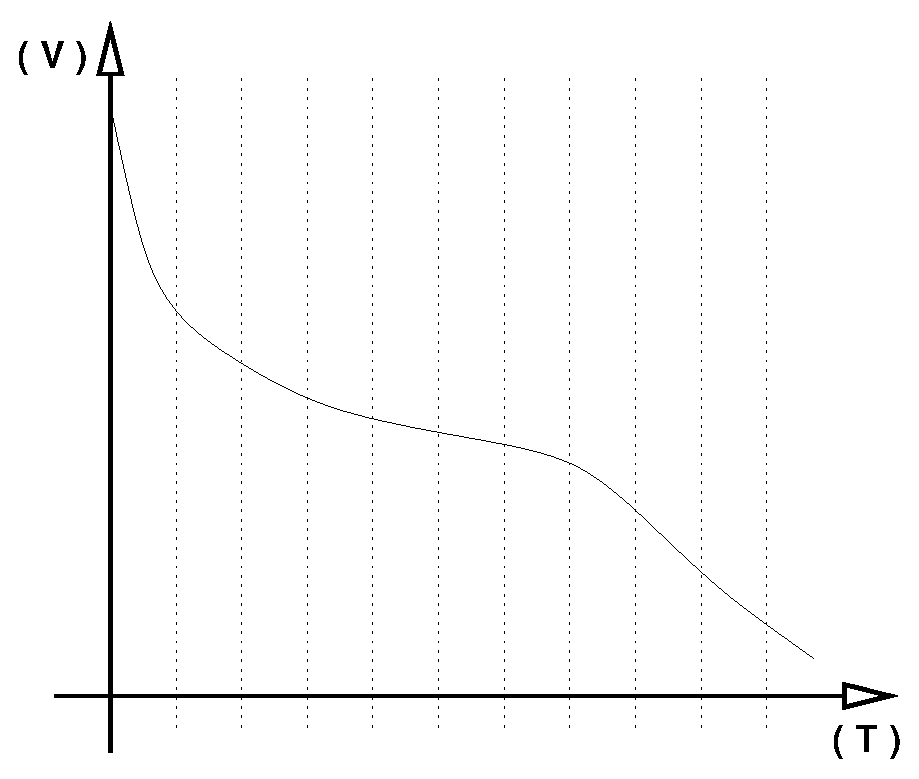
\includegraphics[scale=0.5]{figuras/graficoBateria.eps}}
     \caption{Voltage X Time graphic.}
     \label{fig:graficoBateria}
\end{figure}
%Determinados sistemas embarcados possuem a possibilidade de configurar um
%perfif�rico, chamado conversor anal�gico digital(\textsc{ADC}), para realizar
%as leituras da tens�o da bateria.

%O monitor do \epos{} n�o realiza um acompanhamento constante da tens�o real da bateria, apesar disso ser poss�vel, pois cada leitura consome energia para ser realizada, al�m de um \ov{} consider�vel para a aplica��o. Para diminuir esses efeitos, o monitor utiliza uma estrutura com informa��es conhecidas previamente que permite acompanhar o consumo de energia de uma forma aproximada. As informa��es s�o a respeito das caracter�sticas espec�ficas da bateria e dos consumos de energia pelos componentes de \emph{hardware} do sistema a ser monitorado. No in�cio da execu��o o monitor verifica a carga da bateria atrav�s da tens�o, como mencionado anteriormente, e durante a execu��o atualiza esse valor com as energias consumidas pelos perif�ricos do sistema.

The \epos{} monitor does not implement a constant tracking of the real battery
voltage, as each sampling consumes energy to be
realized, in addition to considerably overhead for the application. In order to
reduce these effects, the monitor uses a structure with information previously
known which allows tracking the energy consumption in an approximate way. The
information are in relation to specific characteristics of the battery and
energy consumption by the system hardware components that will be monitored. The
monitor verifies the battery charge through the voltage in the beginning of the
execution, and during the execution updates the value
with energy consumed by system peripherals.


%- Explicar sobre a implementa��o da computa��o imprecisa no \epos{}. (2 ou 3 par�grafos, colocar alguma figura aqui - diagramas de classe) Explicar tamb�m que � poss�vel cancelar a parte obrigat�ria no meio, aplica��o fica respons�vel de assegurar a validade dos dados computados pela parte opcional. Possibilidades: colocar bits de controle ou mesmo \emph{timestamp} da �ltima atualiza��o dos dados.

%As caracter�sticas e as funcionalidades do \epos{} apresentadas s�o vantajosas para a nossa proposta. A partir disso, n�s estendemos o \epos{} para suportar o nosso algoritmo de escalonamento com tarefas imprecisas e execu��es condicionais aos par�metros desejados (tempo e energia).


%The \epos{} features and functionality presented are advantageous to our
%proposal. Thus, we extended \epos{} to support our scheduler algorithm with
%imprecise tasks and conditional executions to desired parameters, i.e., time and
%energy.



%As tarefas imprecisas no \epos{} foram modeladas com base nas fun��es monot�nicas da computa��o imprecisa. Nessa modelagem, as fun��es melhoram a qualidade do resultado durante o tempo que permanecem executando e na pior das hip�teses n�o alteram o resultado, ou seja, a parte obrigat�ria retorna a solu��o com o m�nimo de \qos{} necess�ria para a continuidade da aplica��o e a parte opcional faz refinamentos sucessivos nessa solu��o. O t�rmino dessas fun��es pode ocorrer em qualquer momento da execu��o sem ocasionar problemas de integridade no resultado, assim sendo, o escalonador pode decidir em qualquer instante finalizar a execu��o da parte opcional. A aplica��o fica respons�vel pela integridade dos resultados atrav�s de diferentes m�todos, como o uso de bits de controle ou mesmo o uso de \emph{timestamps} da �ltima atualiza��o dos dados. 

We extended \epos{} to support our scheduler algorithm with
imprecise tasks and conditional executions to desired parameters, i.e., time and
energy.
The tasks model in \epos{} was based on monotone imprecise tasks. In this
model, the monotone tasks improve the result quality at the time in
execution and the worst case do not change the result. Thus, the mandatory
subtasks generate results with the minimum \qos{} necessary to guarantee
that these results are useful, and the optional subtasks realize successive
refinements that results. The completion of these tasks can occur at any
execution time without cause integrity problems in the results. Therefore, the
scheduler can decide at any instant to finalize the optional subtask execution.
The application is responsible for the results integrity by different methods
such as the use of control bits or the use of last data update timestamps.


%A implementa��o das tarefas imprecisas no \epos{} foi realizada atrav�s da cria��o de duas \emph{threads}, uma contendo o fluxo de execu��o da parte obrigat�ria e outra com o fluxo de execu��o da parte opcional. O sistema cria essas \emph{threads} de uma forma transparente para o programador da aplica��o. Essa abordagem apenas espera que o programador especifique, no momento da cria��o de uma tarefa imprecisa, dois ponteiros para fun��es: um para a parte obrigat�ria e outro para a parte opcional, com os seus respectivos par�metros.

The imprecise tasks implementation in \epos{} was realized through the creation
of two threads: one containing execution flow to handle the mandatory part and
another with the execution flow to handle the optional part. The system
creates these threads in a transparent manner to the application programmer.
This approach only expects the programmer to specify, when creating a imprecise 
thread, two entry points: one for the mandatory subtask and another
for the optional subtask with their parameters.


%Na execu��o, o escalonador escolhe sempre a parte de mais alta prioridade de acordo com o nosso algoritmo baseado no \textsc{EDF}. As partes opcionais s�o escalonadas quando n�o existirem partes obrigat�rias com o estado \textit{Pronto} e se houver energia, ou seja, as partes opcionais possuem prioridades inferiores as partes obrigat�rias. Caso uma parte obrigat�ria entre no estado \textit{Pronto} e sua parte opcional ainda n�o tenha terminado de executar no per�odo anterior, o escalonador imediatamente finaliza a execu��o da parte opcional. Essas caracter�sticas fazem com que n�o ocorram perdas dos \deadlines{} das partes obrigat�rias. O contexto da parte opcional � sempre reiniciado quando ela sai do estado \textit{Pronto} e entra no estado \textit{Esperando}.

The scheduler in execution always chooses the highest priority subtask in
accordance with the deadlines as our algorithm is based in \textsc{EDF}. The
optional subtasks are scheduled if there are not mandatory subtasks in
\textit{READY} state and if there is energy enough to meet battery lifetime
specified by the application, i.e., optional subtasks have lower priorities than
mandatory subtasks. When a mandatory subtask enters in \textit{READY} state and
its optional subtask is not yet finished the execution in the previous period,
the scheduler immediately suspends this optional subtask execution. These
characteristics prevent mandatory subtasks deadlines losses. The optional
subtasks contexts are always restarted in a new task period.
%when they leave the \textit{READY} state and enter in \textit{WAITING} state.


%O escalonador tamb�m atualiza, em tempo de execu��o, o $T_{t \kappa}$ com o tempo decorrido no sistema e o $E_{t \kappa}$ com a utiliza��o do monitor de energia do \epos{}. Com essas vari�veis atualizadas, o escalonador realimenta a equa��o (\ref{eq:escalonador:ek}) em per�odos $\pi$ de tempos para determinar se o sistema � capaz de manter a carga de trabalho sem que a bateria termine antes de $T_{t \kappa}$ seja alcan�ado. $\pi$ ir� depender do resultado da �ltima an�lise de energia. No melhor caso, a equa��o (\ref{eq:escalonador:ek}) � atendida e todas as partes das tarefas podem ser executadas. Caso contr�rio, as partes opcionais ser�o descartadas e o escalonador executa (nesses intervalos que as partes opcionais estariam em execu��o) o gerente de energia do \epos{} que encontra-se no modo passivo. Nesse caso, al�m da economia de energia por n�o executar as partes opcionais, o gerente reduz o consumo global do sistema atrav�s do uso de t�cnicas de ger�ncia de energia. No instante $\kappa+\iota$ em que o escalonador identifique que $T_{t \kappa+\iota}$ pode ser alcan�ado novamente, o sistema volta a permitir a execu��o das partes opcionais. 

The scheduler also updates at execution-time the $T_{t \kappa}$ with elapsed
time and the $E_{t \kappa}$ using the \epos{} energy monitor. Scheduler
recalculates the equation (\ref{eq:escalonador:ek}) in periods $\pi$ with these
new values in order to check if the system is able to sustain the current
workload without running out of battery before the required lifetime $T_{t
\kappa}$ is achieved. $\pi$ will depend on the last energy analysis. In the best
case, equation (\ref{eq:escalonador:ek}) is respected and all parts of the tasks
can be executed. Otherwise, optional subtasks are discarded and, taking
advantage of the idle period created, the scheduler executes the \epos{} power
manager in passive mode. In addition to saving energy by not execute the
optional subtasks, the power manager reduces the system energy consumption
through the use of power management techniques. The optional subtasks return to
execution when the scheduler identify $T_{t \kappa+\iota}$ can be met again in
instant $\kappa+\iota$.


%- Diagrama de sequencia seria interessante




% Summary 

% Contributions: (1) common and simple interface (minor), (2)
% Power-management on embedded systems without using any complex
% high-cost methodology.
In this paper we presented an strategy to enable application-driven
power management in deeply embedded systems. In order to achieve this
goal we allowed application programmers to express when certain
components are not being used. This is expressed through a simple
power management interface which allows power mode switching of system
components, subsystems or the system as a whole, making all
combinations of components operating modes feasible. By using the
hierarchical architecture by which system components are organized in
our system, effective power management was achieved for deeply
embedded systems without the need for costly techniques or strategies,
thus incurring in no unnecessary processing or memory overheads.

A case study using a 8-bit microcontroller to monitor temperature in
an indoor ambient showed that almost 40\% of energy could be saved
when using this strategy. % and with minimal application intervention.

% Problems: concurrence. Describe the Thread problem.

% The paper also listed some identified problems on the path for
% power-aware software and hardware components, discussing and
% explaining how some of these problems have been solved in this work
% and how some of them can be solved, and will be, in future work.

% Even so, it still have its usability.





\bibliographystyle{sbc}
\bibliography{bibs/powerManager,bibs/hardware,bibs/impreciseComputations,bibs/lisha,bibs/wsn,bibs/os,bibs/rt,bibs/minhas}

\end{document}
